\documentclass[aspectratio=169]{beamer}
\usetheme{metropolis}
\usepackage[utf8]{inputenc}
\usepackage[T1]{fontenc}
\usepackage{lmodern}
\usepackage{amsmath,amssymb,mathtools}
\usepackage{bm}
\usepackage{tikz}
\usepackage{booktabs}
\usepackage{graphicx}
\usepackage{hyperref}
\usepackage{caption}
\usepackage{minted} % compile with -shell-escape
\setminted{fontsize=\footnotesize, breaklines, autogobble, frame=lines}

\title{KAN Tutorial Slides}
\author{Daniel Precioso Garcelán}
\date{\today}
\begin{document}
\maketitle
\begin{frame}{Kolmogorov-Arnold Networks}

\end{frame}

\begin{frame}{Kolmogorov-Arnold Representation Theorem}
Let $ \Omega \subset \mathbb{R}^d $ be a bounded domain and let $ f: \Omega \rightarrow \mathbb{R} $ be a continuous function; i.e. $ f \in C(\Omega) $.

Then there exist continuous univariate functions
$$
\Phi_q: \mathbb{R} \to \mathbb{R}, \quad q = 1, \dots, 2d+1;
$$
and continuous univariate functions
$$
\phi_{pq}: \mathbb{R} \to \mathbb{R}, \quad p = 1, \dots, d; \quad q = 1, \dots, 2d+1;
$$
such that for every $\mathbf{x} = (x_1, \dots, x_d) \in \Omega$,
$$
f(\mathbf{x}) = \sum_{q=1}^{2d+1} \Phi_q \left( \sum_{p=1}^d \phi_{pq}(x_p) \right).
$$
\end{frame}

\begin{frame}{Kolmogorov-Arnold Representation Theorem}
For a bivariate function $f(x_1, x_2)$, we then have:

\begin{figure}
	\centering
	\resizebox{0.4\linewidth}{!}{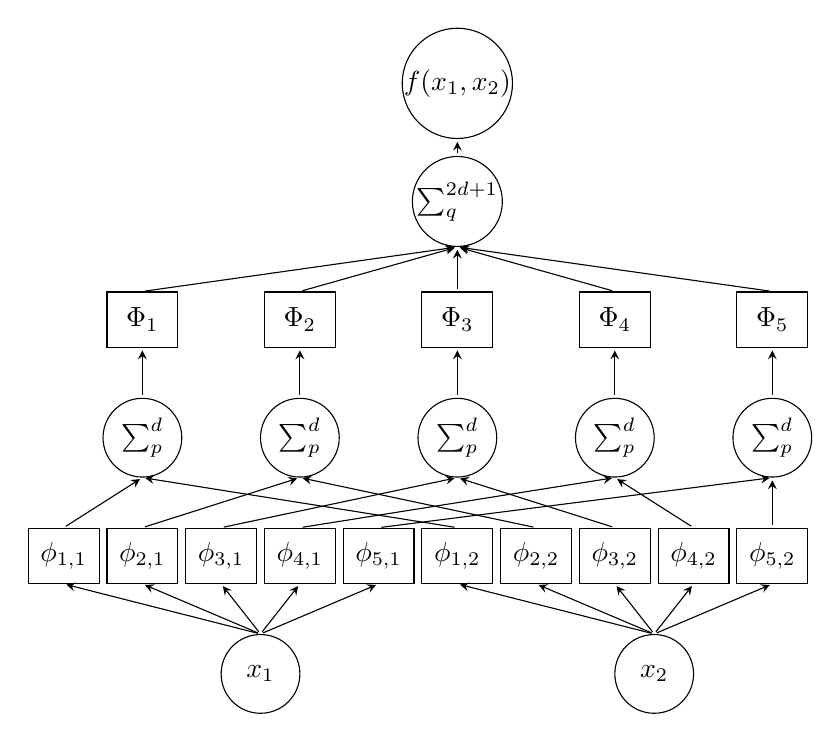
\begin{tikzpicture}[
	neuron/.style={circle, draw, minimum size=10mm, inner sep=0pt},
	box/.style={draw, rectangle, minimum width=9mm, minimum height=7mm, inner sep=1pt, fill=white},
	>=stealth
	]
	
	%-----------------------
	% Customizable heights
	%-----------------------
	\def\hin{0}      % Row 1: inputs
	\def\hphi{1.5}   % Row 2: phi_{i,j} squares
	\def\hsum{3}     % Row 3: per-column sums
	\def\hPhi{4.5}   % Row 4: Phi_j squares
	\def\hsumall{6}  % Row 5: global sum
	\def\hout{7.5}   % Row 6: output
	
	%-----------------------
	% Row 1: inputs
	%-----------------------
	\node[neuron] (X1) at (-2.5,\hin) {$x_1$};
	\node[neuron] (X2) at ( 2.5,\hin) {$x_2$};
	
	%-----------------------
	% Row 2: phi_{i,j} squares
	%-----------------------
	\node[box] (phi1-1) at (-5,\hphi) {$\phi_{1,1}$};
	\node[box] (phi2-1) at (-4,\hphi) {$\phi_{2,1}$};
	\node[box] (phi3-1) at (-3,\hphi) {$\phi_{3,1}$};
	\node[box] (phi4-1) at (-2,\hphi) {$\phi_{4,1}$};
	\node[box] (phi5-1) at (-1,\hphi) {$\phi_{5,1}$};
	
	\node[box] (phi1-2) at (0,\hphi) {$\phi_{1,2}$};
	\node[box] (phi2-2) at (1,\hphi) {$\phi_{2,2}$};
	\node[box] (phi3-2) at (2,\hphi) {$\phi_{3,2}$};
	\node[box] (phi4-2) at (3,\hphi) {$\phi_{4,2}$};
	\node[box] (phi5-2) at (4,\hphi) {$\phi_{5,2}$};
	
	%-----------------------
	% Row 3: per-column sums
	%-----------------------
	\node[neuron] (S-1) at (-4,\hsum) {$\textstyle\sum^d_p$};
	\node[neuron] (S-2) at (-2,\hsum) {$\textstyle\sum^d_p$};
	\node[neuron] (S-3) at ( 0,\hsum) {$\textstyle\sum^d_p$};
	\node[neuron] (S-4) at ( 2,\hsum) {$\textstyle\sum^d_p$};
	\node[neuron] (S-5) at ( 4,\hsum) {$\textstyle\sum^d_p$};
	
	%-----------------------
	% Row 4: Phi_j squares
	%-----------------------
	\node[box] (Phi-1) at (-4,\hPhi) {$\Phi_{1}$};
	\node[box] (Phi-2) at (-2,\hPhi) {$\Phi_{2}$};
	\node[box] (Phi-3) at ( 0,\hPhi) {$\Phi_{3}$};
	\node[box] (Phi-4) at ( 2,\hPhi) {$\Phi_{4}$};
	\node[box] (Phi-5) at ( 4,\hPhi) {$\Phi_{5}$};
	
	%-----------------------
	% Row 5: global sum
	%-----------------------
	\node[neuron] (Sall) at (0,\hsumall) {$\textstyle\sum^{2d+1}_q$};
	
	%-----------------------
	% Row 6: output
	%-----------------------
	\node[neuron] (F) at (0,\hout) {$f(x_1,x_2)$};
	
	%-----------------------
	% Connections (use top/bottom anchors)
	%-----------------------
	\tikzset{connect/.style={->,shorten >=1pt,shorten <=1pt}}
	
	% Inputs -> phi (into phi from below)
	\draw[connect] (X1.north) -- (phi1-1.south);
	\draw[connect] (X1.north) -- (phi2-1.south);
	\draw[connect] (X1.north) -- (phi3-1.south);
	\draw[connect] (X1.north) -- (phi4-1.south);
	\draw[connect] (X1.north) -- (phi5-1.south);
	
	\draw[connect] (X2.north) -- (phi1-2.south);
	\draw[connect] (X2.north) -- (phi2-2.south);
	\draw[connect] (X2.north) -- (phi3-2.south);
	\draw[connect] (X2.north) -- (phi4-2.south);
	\draw[connect] (X2.north) -- (phi5-2.south);
	
	% phi -> per-column sums (enter sums from below)
	\draw[connect] (phi1-1.north) -- (S-1.south);
	\draw[connect] (phi1-2.north) -- (S-1.south);
	\draw[connect] (phi2-1.north) -- (S-2.south);
	\draw[connect] (phi2-2.north) -- (S-2.south);
	\draw[connect] (phi3-1.north) -- (S-3.south);
	\draw[connect] (phi3-2.north) -- (S-3.south);
	\draw[connect] (phi4-1.north) -- (S-4.south);
	\draw[connect] (phi4-2.north) -- (S-4.south);
	\draw[connect] (phi5-1.north) -- (S-5.south);
	\draw[connect] (phi5-2.north) -- (S-5.south);
	
	% sums -> Phi (upwards)
	\draw[connect] (S-1.north) -- (Phi-1.south);
	\draw[connect] (S-2.north) -- (Phi-2.south);
	\draw[connect] (S-3.north) -- (Phi-3.south);
	\draw[connect] (S-4.north) -- (Phi-4.south);
	\draw[connect] (S-5.north) -- (Phi-5.south);
	
	% Phi -> global sum
	\draw[connect] (Phi-1.north) -- (Sall.south);
	\draw[connect] (Phi-2.north) -- (Sall.south);
	\draw[connect] (Phi-3.north) -- (Sall.south);
	\draw[connect] (Phi-4.north) -- (Sall.south);
	\draw[connect] (Phi-5.north) -- (Sall.south);
	
	% Global sum -> output
	\draw[connect] (Sall.north) -- (F.south);
	
\end{tikzpicture}}
\end{figure}

Which is a simple KAN!
\end{frame}

\begin{frame}{B-Splines}
$\Phi_q$ and $\phi_{p,q}$ can be chosen from any family of continuous univariate functions. A common choice is the **B-spline** family.

A B-spline of degree $k$ is defined as:

$$B_k(x) = \sum_{i=0}^{n-k-1} P_i N_{i,k}(x)$$

where $n$ is the number of control points (length of the knot vector), and $P_i$ are the basis function weights.

And $N_{i,k}$ are the basis functions, following the standard **Cox-de Boor recursive definition**:

$$
N_{i,0}(x) =
\begin{cases}
1, & t_i \le x < t_{i+1} \\
0, & \text{otherwise}
\end{cases}
$$

$$
N_{i,k}(x) =
\frac{x - t_i}{t_{i+k} - t_i} N_{i,k-1}(x)
+
\frac{t_{i+k+1} - x}{t_{i+k+1} - t_{i+1}} N_{i+1,k-1}(x),
\quad k > 0
$$

where ${t_i} \in [t_1, t_n]$ is the **knot vector**, a non-decreasing sequence of real numbers.
\end{frame}

\begin{frame}{Grid Extension}

\end{frame}

\begin{frame}{Continuous Learning}
B-splines are made of basin functions that operate in small bounds of X. Learning new information in a part of X does not alter other regions of X. In contrary, traditional MLP risk **catastrohpic forgetting**.
\end{frame}

\begin{frame}{Symbolic Regression}

\end{frame}

\begin{frame}{Sparsibility}

\end{frame}

\end{document}
